\documentclass[a4paper, 12pt]{article}

\usepackage[T2A]{fontenc}
\usepackage[utf8]{inputenc}
\usepackage[english,russian]{babel}
\usepackage{listings}
\usepackage{multirow}
\usepackage{pgfplots}
\usepackage{pgfplotstable}
\usepackage[normalem]{ulem}
\usepackage{cmap}
\usepackage{geometry}
\usepackage{amsmath}
\usepackage{titlesec}
\usepackage{graphicx}
\graphicspath{ {data/} }

\usepgfplotslibrary{units}
\usepgfplotslibrary{patchplots}
\pgfplotsset{compat=1.10}
\geometry{left=25mm, right=10mm, top=20mm, bottom=20mm}

\renewcommand{\thepart}{\arabic{part}}
\renewcommand{\thesection}{\thepart.\arabic{section}}

\titleformat{\part}
    {\normalsize\bfseries}
    {ЧАСТЬ \thepart.}
    {1mm}{}

\titleformat{\section}
    {\normalsize\bfseries}
    {\thesection.}
    {1mm}{}

\title{3.1 Титульный лист}

\begin{document}

\thispagestyle{empty}

\begin{center}
    Санкт-Петербургский политехнический университет Петра Великого\\
    Институт компьютерных наук и технологий\\
    \bfseries{Кафедра «Информационные и управляющие системы»}
\end{center}

\vspace{20ex}

\begin{center}
    {
    \LARGE \textbf{КУРСОВОЙ ПРОЕКТ} \\[3ex]
    по дисциплине: «Математические модели» \\
    по теме: «Моделирование процесса параметрической идентификации динамического объекта» \\[3ex]
    Вариант №37
    }
\end{center}

\vspace{40ex}

\noindent Выполнил\\
студент гр.23531/21\hfill
\begin{minipage}{0.7\textwidth}
    \hfill \uline{\hspace{3cm}} \hspace{1.1cm} Д.П. Буканов
\end{minipage}

\vspace{3ex}

\noindent Руководитель,\\
доцент\hfill
\begin{minipage}{0.7\textwidth}
    \hfill \uline{\hspace{3cm}} \hspace{0.5cm} Т.В. Леонтьева
\end{minipage}

\vspace{3ex}

\hfill \begin{minipage}{0.6\textwidth} \hfill «\uline{\hspace{1cm}}»\uline{\hspace{3cm}} 2017 г.\end{minipage}

\vfill

\begin{center}
    Санкт-Петербург\\
    2017
\end{center}

\newpage
\thispagestyle{empty}
\begin{center}
    ЗАДАНИЕ\\
    НА ВЫПОЛНЕНИЕ КУРСОВОГО ПРОЕКТА \\[1ex]
    студенту группы 23531/22 Буканову Д. П.
\end{center}

\vspace{0.5cm}

\begin{enumerate}
    \item
        \textbf{Тема проекта (работы):} Моделирование процесса параметрической идентификации динамического объекта, вариант №37
    \item
        \textbf{Срок сдачи студентом законченного проекта (работы):} 30.12.2017
    \item
        \textbf{Исходные данные к проекту (работе):}
            $$
                W(S) = \frac{k(1-a_1s)(1+a_2s)}{(1+b_1s)(1+b_2s)^2}
            $$
            $$
                \begin{matrix}
                    \begin{aligned}
                        x(t) = const = 2 \\
                        k = 4 \\
                        a_1 = 4 \\
                        a_2 = 6 \\
                        b_1 = 2 \\
                        b_2 = 4
                    \end{aligned}
                    &
                    \hspace{3cm}
                    \begin{aligned}
                        \text{метод оптимизации}&: \text{покоординатный спуск} \\
                        \text{целевая функция}&: \text{2} \\
                        \text{шум}&: \text{3} \\
                        \text{считать неизвестными}&: \text{$a_1, k$} \\
                    \end{aligned}
                \end{matrix}
            $$
    \item
        введение, основная часть (раскрывается структура основной части), заключение, список использованных источников, приложения, нахождение $y^T$, создание и проверка ГСЧ с помощью гистограмм, формирование шума и $y^\epsilon$, реализация алгоритма оптимизации и проверка на тестовых функциях, нахождение $m^M$ и целевой функции $(CF)$, её оптимизация. Примерный объем пояснительной записки 28 страниц машинописного текста
    \item
        \textbf{Консультанты:} Леонтьева Т.В.
    \item
        \textbf{Дата получения задания:} 05 сентября 2017 г.
\end{enumerate}

\vfill

\noindent \textbf{Руководитель} \hfill
\hfill \uline{\hspace{3cm}} \hspace{1.1cm} Леонтьева Т.В.

\vspace{1cm}

\noindent \textbf{Задание принял к исполнению} \hfill
\hfill \uline{\hspace{3cm}} \hspace{1.7cm} Буканов Д.П.

% \newpage
% \tableofcontents

\newpage
\part{НАХОЖДЕНИЕ $y^T$ (ТЕОРЕТИЧЕСКОГО)}
\section{Составление системы дифференциальных уравнений}

$$
    W(s) = \frac{k(1-a_1s)(1+a_2s)}{(1+b_1s)(1+b_2s)^2} = \frac{P(s)}{Q(s)}
$$

\vspace{1cm}

$$
    \begin{cases}
        \dfrac{1}{Q(s)} = \dfrac{u(s)}{x(s)}
        \\\\ % Это зашквар, надо будет поправить
        P(s) = \dfrac{y(s)}{u(s)}
    \end{cases}
    \Rightarrow
    \begin{cases}
        y(s) = k(1-a_1s)(1+a_2s) \cdot u(s)
        \\
        x(s) = (1+b_1s)(1+b_2s)^2 \cdot u(s)
    \end{cases}
$$

\vspace{1cm}

$$
    \begin{aligned}
        y(s)
        &= k(1-a_1s)(1+a_2s) \cdot u(s) \\
        &= k(1 - a_1a_2s^2-a_1s + a_2s) \cdot u(s) \\
        &= ku(s) - ka_1su(s) + ka_2su(s) - ka_1a_2s^2u(s) 
        \\\\
        x(s)
        &= ((1+b_1s)(1+b_2s)^2) \cdot u(s) \\
        &= ((1+b_1s)(1+2b_2s + b_2^2s^2)) \cdot u(s) \\
        &= u(s) + b_1su(s) + 2b_2su(s) + b_2^2s^2u(s) + 2b_1b_2s^2u(s) + b_1b_2^2s^3u(s)
    \end{aligned}
$$

\vspace{1cm}

$$
    \begin{matrix}
        \begin{matrix}
            x(s) \to x(t) \\
            y(s) \to y(t) \\
            u(s) \to u(t) \\
        \end{matrix}
        &
        S = \dfrac{d}{dt}
        &
        S^n = \dfrac{d^n}{dt^n}
    \end{matrix}
$$

\vspace{1cm}

$$
    \begin{aligned}
        y(t) &= ku(t) - ka_1\dot{u}(t) + ka_2\dot{u}(t) - ka_1a_2\ddot{u}(t)
        \\
        x(t) &= u(t) + 2b_2\dot{u}(t) + b_1\dot{u}(t) + b_2^2\ddot{u}(s) + 2b_1b_2\ddot{u}(t) + b_1b_2^2\dddot{u}(t)
    \end{aligned}
$$

\vspace{1cm}

$$
    \begin{aligned}
        \dddot{u}(t)
        &= \frac{1}{b_1b_2^2} \cdot (u(t) + 2b_2\dot{u}(t) + b_1\dot{u}(t) + b_2^2\ddot{u}(t) + 2b_1b_2\ddot{u}(t) - x(t))
        \\
        &= \frac{1}{b_1b_2^2} \cdot \underbrace{u(t) + 2b_2\dot{u}(t) + b_1\dot{u}(t) + b_2^2\ddot{u}(t) + 2b_1b_2\ddot{u}(t) - x(t)}_{\Omega}
    \end{aligned}
$$

\section{Замена переменных в системе дифференциальных уравнений}
$$
    \begin{matrix}
        \begin{aligned}
            z_1(t) = &u(t) &
            \\
            z_2(t) = &\dot{u}(t) = \dot{z_1}(t) &
            \\
            z_3(t) = &\ddot{u}(t) = \dot{z_2}(t) &
            \\
            &\dddot{u}(t) = \dot{z_3}(t) = \Omega &
        \end{aligned}
        &
        \Rightarrow
        &
        \begin{aligned}
            \dot{z_1} &= z_2
            \\
            \dot{z_2} &= z_3
            \\
            \dot{z_3} &= \dfrac{\Omega}{b_1b_2^2}
        \end{aligned}
        &
        \Rightarrow
        &
        \begin{aligned}
        y(t)
        &= k \cdot z_{1} - k \cdot a_1 \cdot a_2 \cdot z_{3} - k \cdot a_1 \cdot z_{2} + k \cdot a_2 \cdot z_{2}
        \\
        &= k \cdot (z_{1} - a_1 \cdot a_2 \cdot z_{3} - a_1 \cdot z_{2} + a_2 \cdot z_{2})
        \end{aligned}
    \end{matrix}
$$

\section{Решение системы методом Эйлера}
$$
    \begin{cases}
        z_{1,n+1} = z_{1,n} + h \cdot z_{2,n}
        \\
        z_{2,n+1} = z_{2,n} + h \cdot z_{3,n}
        \\
        z_{3,n+1} = z_{3,n} + h \cdot \Omega
    \end{cases}
$$

$$
    \begin{aligned}
        y(s)
        &= k \cdot z_{1,n} - k \cdot a_1 \cdot a_2 \cdot z_{3,n} - k \cdot a_1 \cdot z_{2,n} + k \cdot a_2 \cdot z_{2,n}
        \\
        &= k \cdot (z_{1,n} - a_1 \cdot a_2 \cdot z_{3,n} - a_1 \cdot z_{2,n} + a_2 \cdot z_{2,n})
    \end{aligned}
$$

\section{График и таблица значений}

\pgfplotsset{
    gr1/.style = {
        red,
        samples = 100,
        mark = *,
        mark options = {
            scale = 0.1
        },
        line width = 0.5mm
    }
}

\begin{center}
    \begin{tikzpicture}
        \begin{axis}[
            width=16cm,
            height=10cm,
            xlabel=t,
            ylabel=y(t),
            minor tick num = 1,
            grid = both
        ]

        \addplot[color=blue] table {data/points.dat};

        \end{axis}
    \end{tikzpicture}
    \pgfplotstabletypeset[
        col sep=space,
        header=true,
        columns/0/.style = {
            string type,
            column name = $t$
            },
        columns/1/.style = {
            column name=$y(t)$,
            fixed,
            fixed zerofill,
            precision=11,
            dec sep align
        }
    ]{data/points.dat}
\end{center}

\section{Проверка}

При $x(t) = const (C) = 2$ и $k = 4$

$$
    \lim_{s\to0}CW(s) = C \cdot \lim_{s\to0}\left(\dfrac{
        k\overbrace{(1-a_1s)}^{\to1}\overbrace{(1+a_2s)}^{\to1}
    }{
        \underbrace{(1+b_1s)}_{\to1}\underbrace{(1+b_2s)^2}_{\to1}
    }\right) = C \cdot k = 2 \cdot 4 = 8
$$

\section{Часть 2. Проверка алгоритма оптимизации.}
\subsection{Проверка метода оптимизации на функции эллипса}
Видно, что функция стремится к минимум при аргументах стремящимся к (0;0).
\begin{center}
    \begin{tikzpicture}
        \begin{axis}[
            width=16cm,
            height=16cm,
            xlabel=t,
            ylabel=y(t),
            minor tick num = 1,
            grid = both
        ]

            \draw (0,0) circle[radius=2];
            \draw (0,0) circle[radius=5];
            \draw (0,0) circle[radius=10];

            \addplot[color=red] table {data/points2.dat};

        \end{axis}
    \end{tikzpicture}
\end{center}

\subsection{Проверка метода оптимизации на функции Розенброка}
Видно, что функция стремится к минимум при аргументах стремящимся к (1;1).
\begin{center}
    \begin{tikzpicture}
        \begin{axis}[
            width=16cm,
            height=10cm,
            xlabel=t,
            ylabel=y(t),
            minor tick num = 1,
            grid = both
        ]

            \addplot[color=red] table {data/points3.dat};
        \end{axis}
    \end{tikzpicture}
\end{center}


\section{Часть 3. Добавление шума.}
\subsection{Проверка генератора случайных чисел.}

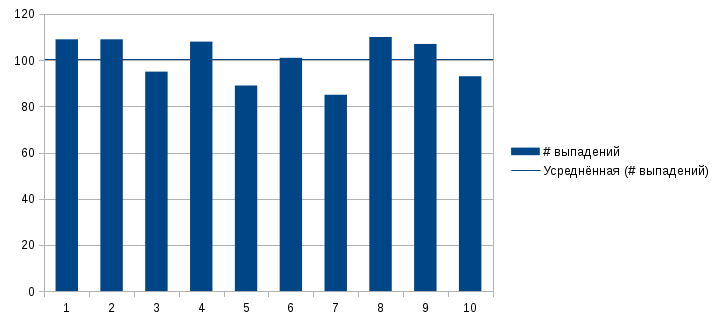
\includegraphics{rnd1}

График показывает, что распределение генерируемых значений близко к Гауссовому.

Шум генерируем по формуле:
$$
\Delta y = max|y(t)| \cdot \begin{Bmatrix}
        0,05 \\
        0,1 \\
        0,2
    \end{Bmatrix} 
$$

$$y(t)_{max} = 7.873587$$

$$
\Delta y = max|y(t)| \cdot \begin{Bmatrix}
        0.39367935 \\
        0.7873587 \\
        1.5747174
    \end{Bmatrix} 
$$

\begin{center}
    \begin{tikzpicture}
        \begin{axis}[
            width=16cm,
            height=10cm,
            xlabel=v,
            ylabel=\#,
            minor tick num = 1,
            grid = both,
            ymin=0
        ]

            \addplot[ybar,fill,color=red] table{data/rnd.dat};
        \end{axis}
    \end{tikzpicture}
\end{center}

Шум

\begin{center}
    \begin{tikzpicture}
        \begin{axis}[
            width=16cm,
            height=10cm,
            xlabel=t,
            ylabel=y(t),
            minor tick num = 1,
            grid = both
        ]

            \addplot[ color=red] table {data/noise/0.dat};
            \addplot[ color=green] table {data/noise/1.dat};
            \addplot[ color=blue] table {data/noise/2.dat};
            \addplot[ color=black] table {data/noise/3.dat};
        \end{axis}
    \end{tikzpicture}
\end{center}

\section{Часть 4.}
$$
\Delta y = \sum_{i=0}^n (Y_i^E - Y_i^m)^2
$$

\begin{center}
    \begin{tikzpicture}
        \begin{axis}[
            width=16cm,
            height=10cm,
            xlabel=t,
            ylabel=y(t),
            minor tick num = 1,
            grid = both
        ]

            \addplot[color=red] table {data/noise/1.dat};
            \addplot[ color=green] table {data/tf/1.dat};
        \end{axis}
    \end{tikzpicture}
\end{center}

\begin{center}
    \begin{tikzpicture}
        \begin{axis}[
            width=16cm,
            height=10cm,
            xlabel=t,
            ylabel=y(t),
            minor tick num = 1,
            grid = both
        ]

            \addplot[color=red] table {data/noise/2.dat};
            \addplot[ color=green] table {data/tf/2.dat};
        \end{axis}
    \end{tikzpicture}
\end{center}

\begin{center}
    \begin{tikzpicture}
        \begin{axis}[
            width=16cm,
            height=10cm,
            xlabel=t,
            ylabel=y(t),
            minor tick num = 1,
            grid = both
        ]

            \addplot[color=red] table {data/noise/3.dat};
            \addplot[ color=green] table {data/tf/3.dat};
        \end{axis}
    \end{tikzpicture}
\end{center}



\end{document}
